\subsubsection{Physical Layer}

This layer creates and deploy the underlying physical connections of the data network and is implemented in the \mintinline{python}{PhysicalLayer} class. 
Types of connections handled by this layer could be ethernet and Wi-Fi links, or even an entire software-defined 4G \gls{LTE} network.

In order to ensure flexibility, we make no assumptions on the wired connections between the data hosts or radios.
On the other hand, an arbitrary data plane could require wired connections between two hosts, or a host and a radio.
Therefore, we use a managed switch at the heart of the physical layer and connect all the hosts and radios to it.
According to the data network description, the physical layer then creates the required \glspl{VLAN} in the switch.

At instantiation time, this class first configures ethernet connections by creating \glspl{VLAN} in the workload data network switch.
It then triggers the deployment of potential wireless connections using \mintinline{python}{WirelessConnection} objects.

A set of \mintinline{python}{WirelessConnection} instances must be provided to the constructor for deployment.
This class can be used as a context manager in a \mintinline{python}{with} statement; at the end of the block, it tears down all connections and cleans the added \glspl{VLAN} from the switch.

\subsubsection{Wireless Connections}
To integrate various wireless connection schemes, we have defined the Python interface \mintinline{python}{WirelessConnection}.
It unifies the interaction of Ainur with the wireless implementation in the following aspects: 
\begin{enumerate}
    \item \textbf{\mintinline{python}{start()} and \mintinline{python}{stop()} methods:} In addition to the constructor and destructor, the implementations need to override these methods which could be called by the \mintinline{python}{PhysicalLayer}.
    The constructor is used to set the configurations by the user and these methods handle the deployment.

    \item \textbf{Data gates:} Every wireless connection implementation must identify certain network interfaces whether on radios or hosts, to act as the gate for the data plane.
    Hence, any host can exchange packets through those gates if the appropriate VLANs are created on the data network managed switch.
\end{enumerate}

Currently, Wi-Fi and \gls{LTE} implementations are available.
User-defined implementation for other wireless connections are possible and encouraged.

We introduce how the current implementations work in the following.

\begin{description}[style=nextline]
    \item[SDR-based Wi-Fi Network]
    The \mintinline{python}{SDRWifi} class handles the configuration and deployment of a software-defined IEEE 802.11 network using the Mangocomm software package and its supported software-defined radios \footnote{See https://mangocomm.com/802.11-mac-phy/}.
    It lunches a Docker container on the same machine to communicate with the \glspl{SDR} over the control network.
    This communication is for the configuration and monitoring the Wi-Fi nodes.
    In a Wi-Fi network, a radio is either \emph{station} or \emph{access point}.
    To initialize a \mintinline{python}{SDRWifi} class, the user is required to provide two lists containing the access points and station nodes instances as described below.
    
    \mintinline{python}{APSoftwareDefinedRadio} class represents a Wi-Fi access point.
    It advertises a network with a specific SSID on a radio channel and waits for the incoming connections.

    \mintinline{python}{StationSoftwareDefinedRadio} class is used for the station Wi-Fi nodes.
    It searches for an Wi-Fi \gls{SSID} among the networks that are being advertised and attempts for establishing the connection.
    
    When a Wi-Fi network is up and an station is connected, the data network interfaces of the radios behave as if an ethernet cable is connecting them.
    Thus, the client hosts and the server hosts can be on the same ip layer subnets.
    \begin{figure}[t]
        \centering
        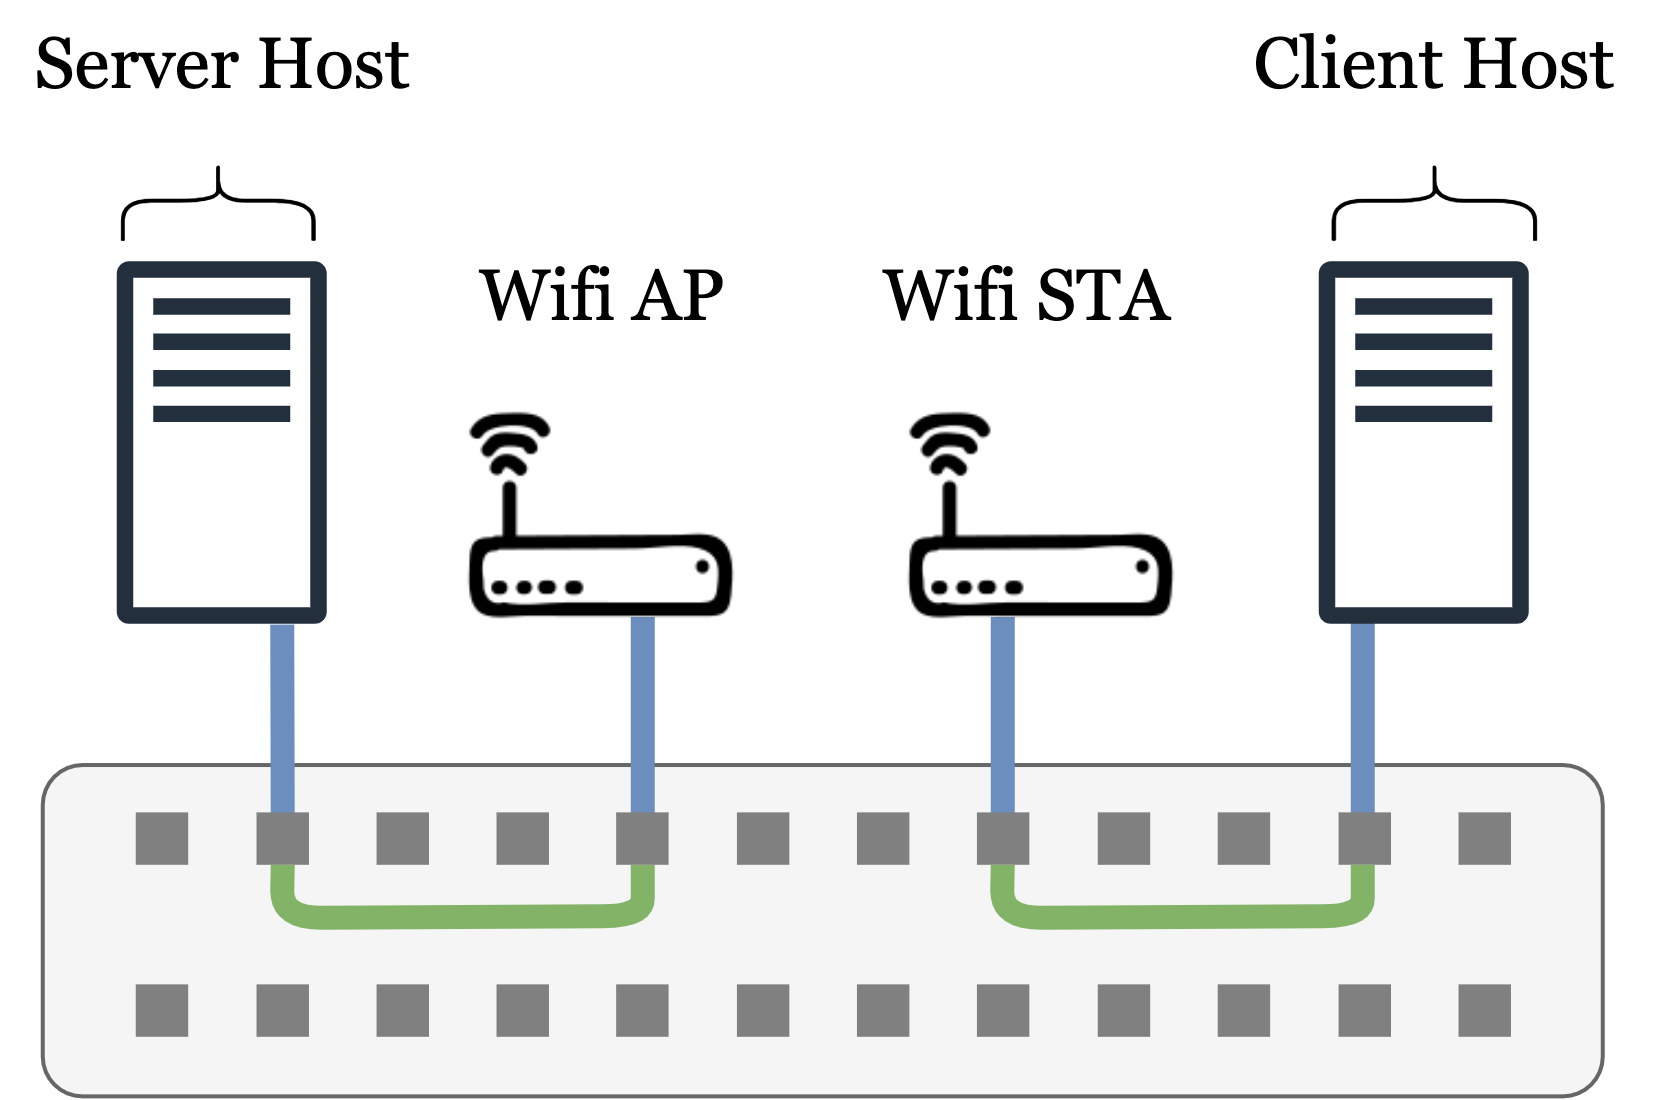
\includegraphics[width=0.8\linewidth]{figures/wifi.png}
        \caption{An example of Wi-Fi network topology in data network and its corresponding \glspl{VLAN}}
        \label{fig:wifi}
    \end{figure}

    \item[\gls{SDR}-based \gls{LTE} Network]
    \mintinline{python}{SDRLTE} class can configure and deploy a complete software-defined \gls{LTE} network.
    The constructor must be provided with an \mintinline{python}{EPC} class, a set of \mintinline{python}{ENodeB} classes, and a set of \mintinline{python}{LTEUE} classes from the \emph{autoran} Python package\footnote{See https://github.com/samiemostafavi/autoran}.
    This package exploits the \emph{docker-py} framework to run containerized OpenAirInterface \gls{LTE} functions on remote hosts.
    Network configurations are needed in the form of Python dictionaries for the construction of \emph{autoran} classes.

    \gls{LTE} \gls{EPC} consists of HSS, MME, SPGW-U, and SPGW-C services which can be run on the same host.
    For each \gls{eNodeB} or \gls{UE}, a software-defined radio and a host for signal processing must be specified additionally.
    The resulting topology of an \gls{LTE} network in Ainur is depicted in Figure \ref{fig:lte}.
    Unlike Wi-Fi wireless connection, due to the fact that \gls{LTE} creates an internal ip network and that introduces routing complexities, the server host and the client host cannot be on the same subnet in the ip layer.
    

    \begin{figure}[t]
        \centering
        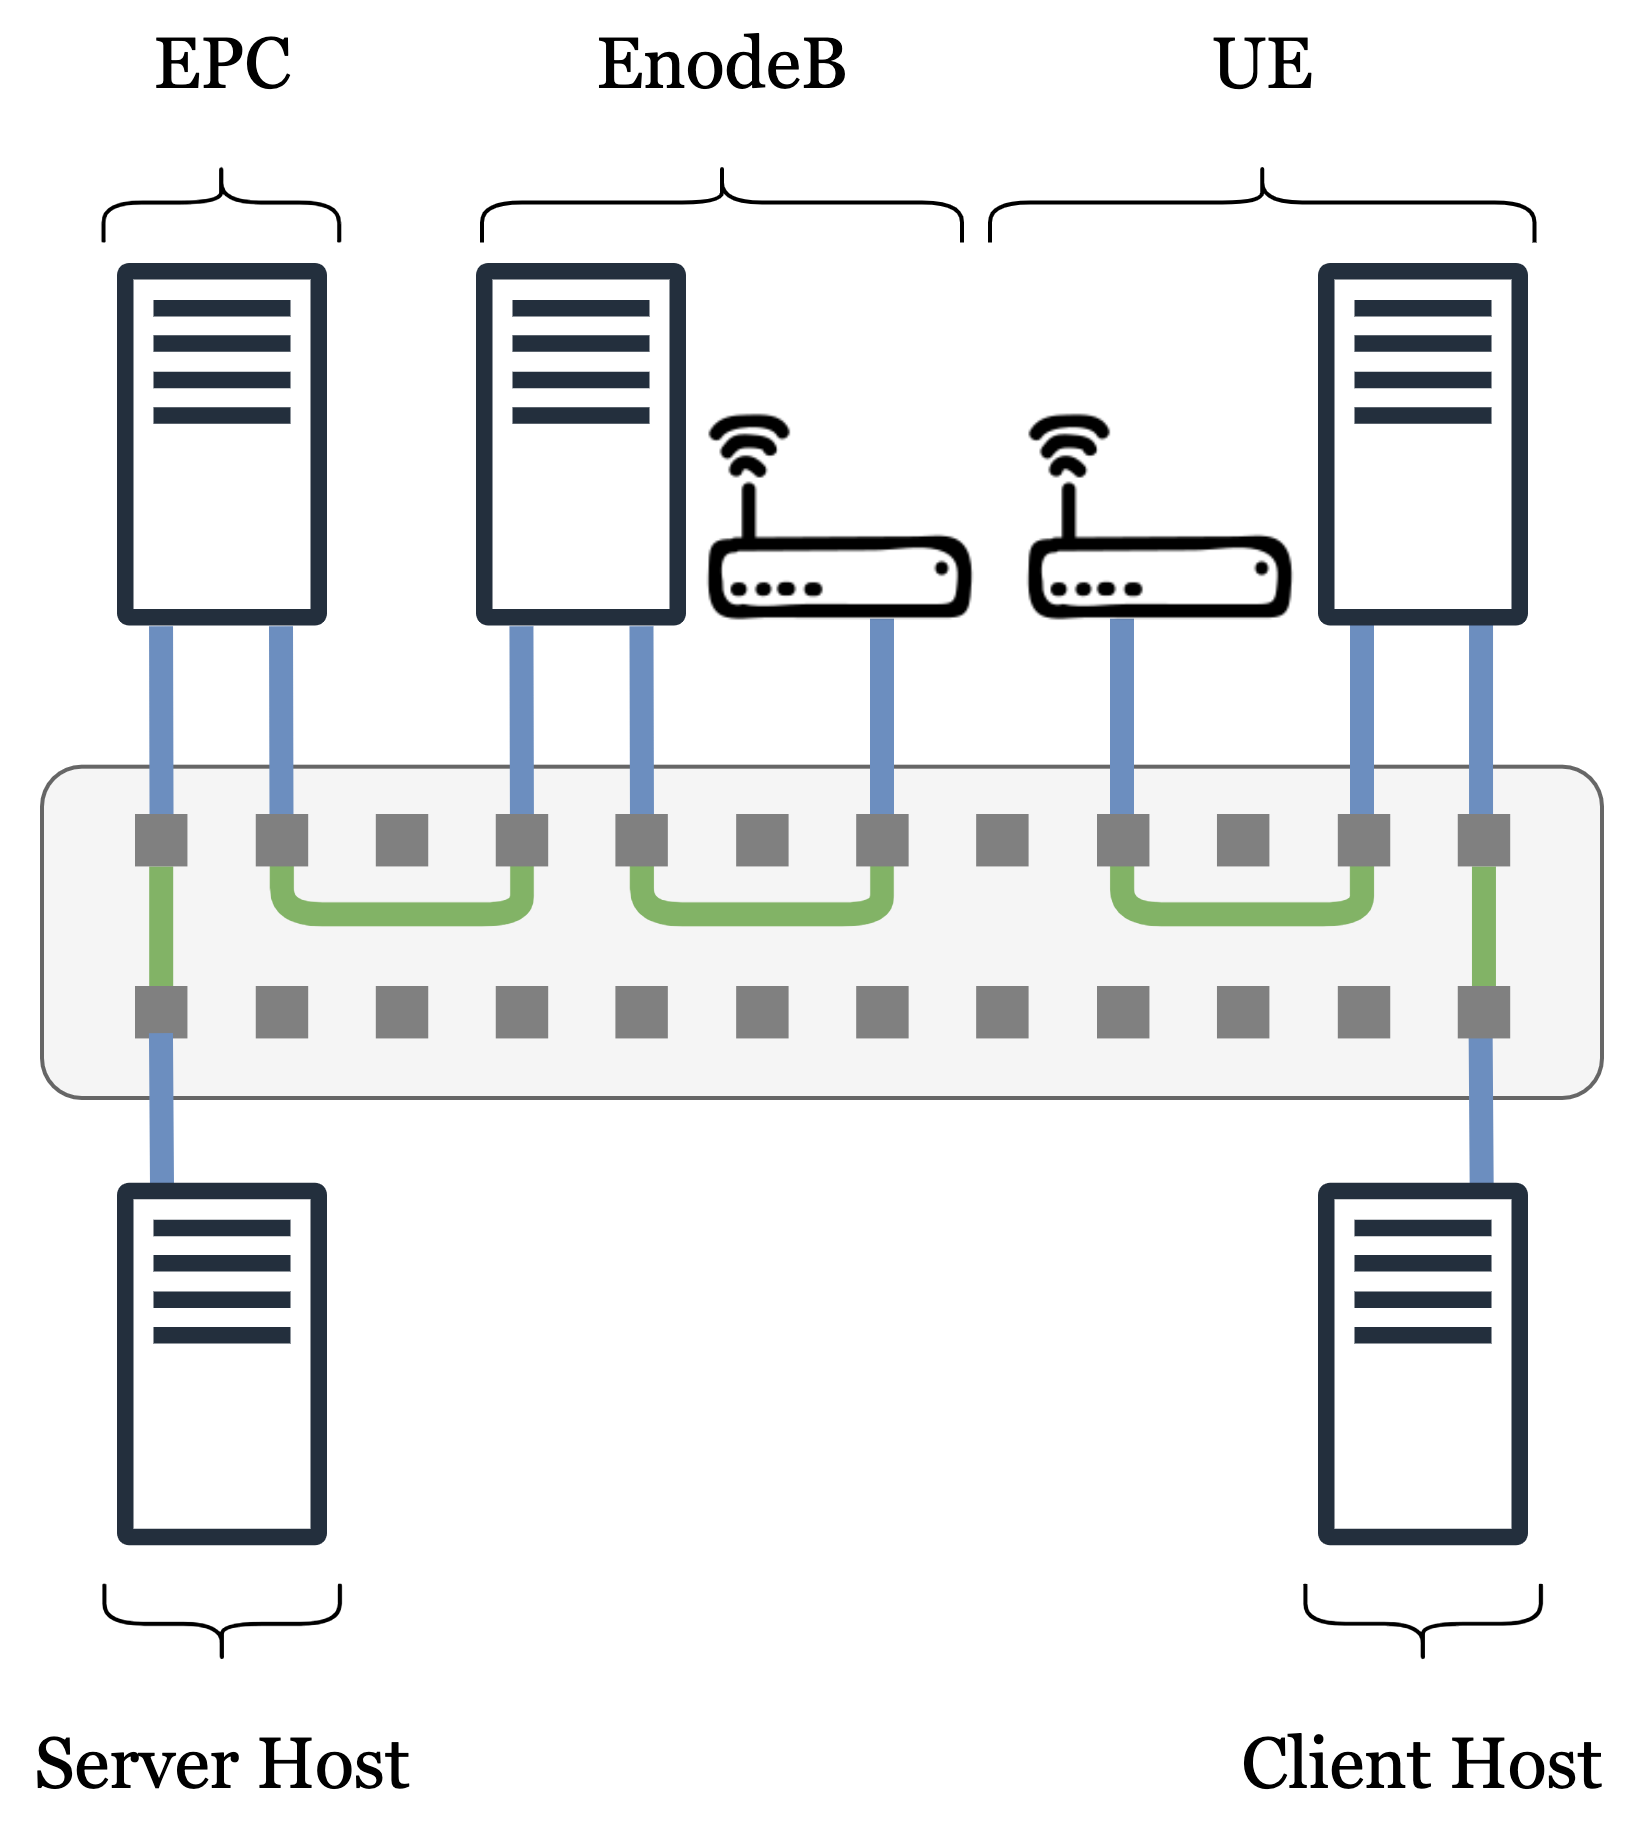
\includegraphics[width=0.8\linewidth]{figures/lte.png}
        \caption{An example of \gls{LTE} data network topology in data network and its corresponding \glspl{VLAN}}
        \label{fig:lte}
    \end{figure}




\end{description}
